\documentclass[10pt,twocolumn]{article}

\usepackage[margin=0.85in]{geometry}
\usepackage{times}
\usepackage{microtype}
\usepackage{booktabs}
\usepackage{amsmath}
\usepackage{graphicx}
\usepackage{xcolor}
\usepackage{pgfplots}
\pgfplotsset{compat=1.17}
\usepackage{titlesec}
\usepackage[hidelinks]{hyperref}
\usepackage{enumitem}
\setlist{nosep,leftmargin=1.2em}

\titleformat{\section}{\normalfont\large\bfseries}{\thesection}{0.6em}{}
\titleformat{\subsection}{\normalfont\normalsize\bfseries}{\thesubsection}{0.6em}{}
\titlespacing*{\section}{0pt}{1.4ex}{0.8ex}
\titlespacing*{\subsection}{0pt}{1.0ex}{0.5ex}

\newcommand{\best}[1]{\textbf{#1}}

\date{September 2026}

\begin{document}

\twocolumn[
\begin{@twocolumnfalse}
\begin{center}
{\LARGE\bfseries A Tiny Model Beats Its Teacher:\\[2pt]
Verified-Loop Repair with a Sub-1B Language Model\par}
\vspace{8pt}
{\large Tanvir Ahmed\par}
\vspace{3pt}
{\small \texttt{github.com/mailtotanvir/nano-agent}\par}
\vspace{12pt}
\begin{minipage}{0.86\textwidth}
\small
\textbf{Abstract.} We show that a 0.5B-parameter code model, placed inside a
deterministic verify--propose--apply--reverify loop whose oracle is the Rust
compiler, repairs compiler errors at rates that exceed the mid-tier model used
to generate its training data. An untrained 0.5B in the loop repairs 0\% of a
frozen 45-case in-distribution set; one round of supervised fine-tuning (SFT) on
348 compiler-verified teacher trajectories lifts this to 86.7\%, edging past the
teacher's own 84.4\% one-shot score. On a frozen, hand-authored 25-case
out-of-distribution (OOD) set the same model scores only 44\%, exposing
overfitting to single-site edits. A failure-driven curriculum---distilling the
\emph{failing skill classes} (never the test cases) from the teacher---raises OOD
accuracy to 60\%, crossing the teacher's 56\% bar. Distilling the same classes
from a stronger (frontier, 100\% OOD) teacher raises it further to 72\%, but the
gain is bounded: residual failures cluster in a single structural class
(insert-whole-method / insert-import), a capacity signal rather than a data gap.
All models run through an identical controller and verifier; the entire study,
including four GPU training rounds, cost under \$6. We argue the recipe
(cheap proposer + perfect verifier + bounded retry + escalation), not the model,
is the artifact.
\vspace{10pt}
\end{minipage}
\end{center}
\end{@twocolumnfalse}
]

\section{Introduction}

The prevailing way to evaluate small language models treats the model as the
product: a single call, in isolation, scored against a benchmark. Under that
framing sub-billion-parameter models look hopeless, and the field concludes they
are unfit for tasks requiring correctness. But almost nothing is deployed as a
raw model. Systems ship a model wrapped in tools, retries, and---crucially---a
check on the work.

A large class of software failures are not open-ended reasoning problems. They
are \emph{bounded and structurally identifiable}: the compiler has already
localized the fault and named its class. The task is not to be brilliant but to
make a correct small edit, in a valid format, and prove it compiles. Where a
cheap, perfect oracle for correctness exists, we hypothesize that a tiny model
inside a verified loop can close most of the gap to a frontier model, at a
fraction of the cost and latency, and without the code ever leaving local
infrastructure.

We test this on Rust compiler-error repair, using \texttt{cargo check} as the
verifier. Our contributions are: (1) a clean 0\% floor that isolates SFT gain
from harness effects; (2) evidence that a nano model can \emph{surpass its own
teacher} on held-out cases; (3) a failure-driven curriculum method that lifts OOD
generalization without touching the frozen eval; and (4) a teacher-strength
ablation that separates a data lever from a capacity ceiling.

\section{Method}

\subsection{The verified repair loop}

The controller is deliberately minimal: no planner, no tool selection. Given a
broken crate, it runs \texttt{cargo check}; if compilation fails, it builds a
context from the rendered primary diagnostic, the file, and the surrounding code,
and asks the model for a patch. Patches use a \textsc{search}/\textsc{replace}
block format rather than a unified diff, because sub-1B models reliably mangle
diff headers and line arithmetic; a GBNF grammar constrains the model to valid
contract JSON. The patch is applied and the crate re-verified. The loop repeats
up to a bounded budget (4 attempts), then escalates to a frontier model. The same
controller, parser, and verifier are used for every arm, including the teacher,
so all trajectories are shape-identical and every step is compiler-checked.

\subsection{Model and training}

The base is Qwen2.5-Coder-0.5B-Instruct, chosen because it is code-pretrained
(it already knows Rust syntax and diagnostic shape), instruct-tuned (it follows a
system prompt and emits structured output), and quantizes to a $\sim$600\,MB q8\_0
GGUF that serves patches in seconds on a 4-core ARM CPU with no GPU. We fine-tune
in full bf16 (no LoRA; a sub-1B model fits comfortably in a single 24\,GB L4),
3 epochs, learning rate $1\times10^{-5}$ with cosine schedule, effective batch 16,
and \texttt{assistant\_only\_loss} so loss is computed only on the JSON patch
target and never on the prompt.

\subsection{Data generation}

Every training example is generated then confirmed by the real compiler before
admission. A parametric seed generator synthesizes compiling Rust programs; a
mutator (\texttt{break\_it.py}) applies a labeled single-site mutation targeting a
specific error class (E0308, E0433, E0599, E0425, E0277, E0596, E0282, E0560, and
syntax); a candidate is kept only if \texttt{cargo check} fails with the intended
code. A stratified, leak-checked split freezes the evaluation set first (case IDs
are content hashes), and the teacher runs the train pool through the same
controller; only successful, compiler-verified episodes become SFT positives.

\subsection{Evaluation sets (frozen)}

\texttt{eval\_v1} is 45 in-distribution cases (single-site mutations).
\texttt{eval\_ood\_v1} is 25 hand-authored out-of-distribution cases: idiomatic
Rust and error categories the mutator never produces (borrow, error handling,
trait bounds, non-exhaustive matches, argument count, missing methods, lifetimes,
float/int mixing). Both are frozen and verified disjoint from all training data
by content hash. We never train on them.

\section{Results}

\subsection{The 0\% floor and the in-distribution result}

Table~\ref{tab:indist} gives the in-distribution results. The untrained 0.5B in
the loop scores 0/45: it obeys the JSON contract but does not emit the
\textsc{search}/\textsc{replace} block, so no patch applies. The identical parser
scores the teacher 38/45, proving the 0\% is the model, not the harness. One SFT
pass closes the entire gap and edges past the teacher, running fully on CPU.

\begin{table*}[t]
\centering
\small
\begin{minipage}[t]{0.46\textwidth}
\centering
\caption{Frozen \texttt{eval\_v1} (45 in-distribution cases). All arms use the
identical controller and \texttt{cargo check} verifier.}
\label{tab:indist}
\begin{tabular}{@{}lcc@{}}
\toprule
Arm & Repair rate & Avg.\ att. \\
\midrule
Untrained 0.5B (loop)        & 0.0\% (0/45)  & 3.89 \\
Gemini Flash (1-shot teacher) & 84.4\% (38/45) & 1.0 \\
\best{Trained 0.5B (SFT v2)} & \best{86.7\% (39/45)} & 1.4 \\
\bottomrule
\end{tabular}
\end{minipage}\hfill
\begin{minipage}[t]{0.5\textwidth}
\centering
\caption{Frozen \texttt{eval\_ood\_v1} (25 held-out cases). Frontier rows are
comparison baselines only; the thesis is a nano model beating its flash-class
\emph{teacher}.}
\label{tab:ood}
\begin{tabular}{@{}lc@{}}
\toprule
Model & OOD rate \\
\midrule
Frontier (1-shot, comparison)          & 100\% (25/25) \\
DeepSeek-V4-Flash (1-shot, comparison) & 84\% (21/25) \\
grok-class (1-shot, comparison)        & 76\% (19/25) \\
Gemini Flash (teacher / the bar)       & 56\% (14/25) \\
Trained 0.5B v2 (single-site SFT)      & 44\% (11/25) \\
Trained 0.5B v3 (+ Flash curriculum)   & 60\% (15/25) \\
\best{Trained 0.5B v4 (+ frontier curr.)} & \best{72\% (18/25)} \\
\bottomrule
\end{tabular}
\end{minipage}
\end{table*}

\subsection{The overfitting gap and the curriculum}

The 86.7\% model scores only 44\% on the frozen OOD set: the single-site-edit
skill memorized a pattern rather than generalizing. We respond with a
failure-driven curriculum. We read the frozen eval's failures, identify the
skill \emph{classes} that fail, and generate fresh, harder cases for exactly
those classes with a structural generator that produces multi-line bugs the
single-site mutator cannot. Critically, we never train on the test; we train on
new instances of the skill the test measures, verified disjoint by hash. This
lifts OOD accuracy from 44\% to 60\% (SFT v3), crossing the teacher's 56\% bar,
with zero regressions on prior wins.

\subsection{Teacher-strength ablation}

To ask whether 60\% is capped by the model or the teacher, we regenerate the same
ten failing classes (250 new verified cases) from a frontier teacher scoring
100\% on the OOD set, merge to 739 SFT examples, and retrain. OOD rises to 72\%
(SFT v4), now +16 points over the flash-teacher bar (Table~\ref{tab:ood};
Figure~\ref{fig:crossover}). A
stronger teacher is therefore a real lever on structural generalization---but a
bounded one.

\begin{figure*}[t]
\centering
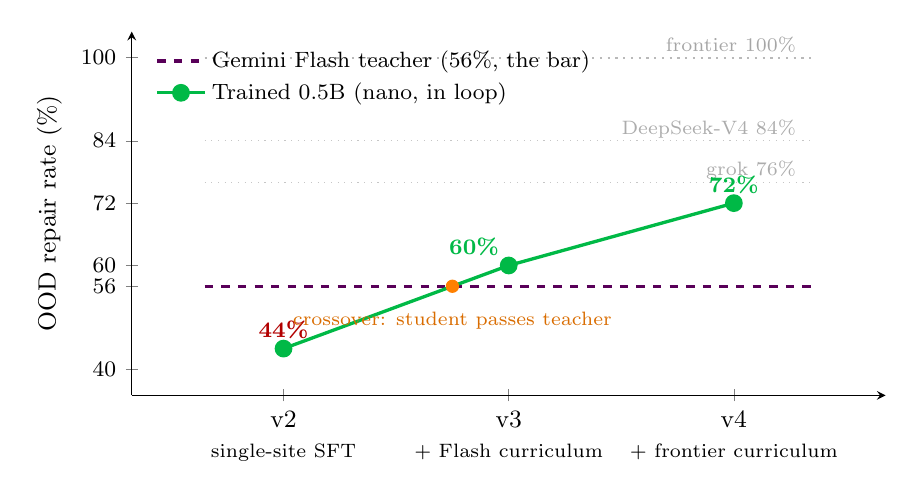
\begin{tikzpicture}
\begin{axis}[
    width=0.92\textwidth, height=6.2cm,
    xmin=-0.35, xmax=2.35, ymin=35, ymax=105,
    xtick={0,1,2},
    xticklabels={v2\\{\scriptsize single-site SFT}, v3\\{\scriptsize + Flash curriculum}, v4\\{\scriptsize + frontier curriculum}},
    xticklabel style={align=center, font=\small},
    ylabel={OOD repair rate (\%)},
    ylabel style={font=\small},
    ytick={40,56,60,72,84,100},
    yticklabel style={font=\footnotesize},
    axis lines=left,
    enlarge x limits=0.12,
    clip=false,
    legend style={font=\footnotesize, at={(0.02,0.98)}, anchor=north west, draw=none, fill=none},
    legend cell align=left,
]
% frontier reference lines (faint, dotted)
\addplot[gray!55, dotted, thick, forget plot] coordinates {(-0.35,100) (2.35,100)};
\node[gray!70, font=\scriptsize, anchor=east] at (axis cs:2.32,102.5) {frontier 100\%};
\addplot[gray!45, dotted, forget plot] coordinates {(-0.35,84) (2.35,84)};
\node[gray!65, font=\scriptsize, anchor=east] at (axis cs:2.32,86.3) {DeepSeek-V4 84\%};
\addplot[gray!45, dotted, forget plot] coordinates {(-0.35,76) (2.35,76)};
\node[gray!65, font=\scriptsize, anchor=east] at (axis cs:2.32,78.3) {grok 76\%};
% teacher bar (the line to beat)
\addplot[violet!70!black, dashed, very thick] coordinates {(-0.35,56) (2.35,56)};
\addlegendentry{Gemini Flash teacher (56\%, the bar)}
% nano model line
\addplot[green!45!teal, very thick, mark=*, mark size=2.6pt] coordinates {(0,44) (1,60) (2,72)};
\addlegendentry{Trained 0.5B (nano, in loop)}
% value labels
\node[anchor=south, font=\footnotesize\bfseries, red!70!black] at (axis cs:0,44) {44\%};
\node[anchor=south east, font=\footnotesize\bfseries, green!45!teal] at (axis cs:1,60) {60\%};
\node[anchor=south, font=\footnotesize\bfseries, green!45!teal] at (axis cs:2,72) {72\%};
% crossover marker (nano line meets 56\% between v2 and v3, at x=0.75)
\addplot[orange, only marks, mark=*, mark size=2.2pt] coordinates {(0.75,56)};
\node[orange!85!black, font=\scriptsize, anchor=north] at (axis cs:0.75,53) {crossover: student passes teacher};
\end{axis}
\end{tikzpicture}
\caption{Out-of-distribution repair accuracy across training rounds. The nano
model (green) rises 44\,$\rightarrow$\,60\,$\rightarrow$\,72\% and crosses the
flash-class teacher's flat 56\% bar (violet, dashed) between the v2 and v3
rounds; frontier models are faint reference lines. In-training eval token
accuracy stayed $\sim$0.95 across all rounds, so the climb is coverage, not fit.}
\label{fig:crossover}
\end{figure*}

\subsection{Where the model runs out of room}

Across all rounds the in-training eval token accuracy is essentially flat
($\sim$0.95), while OOD accuracy climbs 44$\rightarrow$60$\rightarrow$72: the fit
did not change, the coverage did. The seven residual v4 failures cluster in one
family---synthesize and insert a whole trait method or missing import in the
correct scope---and survive even a perfect teacher. That consistency is the
signature of a capacity limit rather than a coverage gap, and indicates the next
lever is reinforcement learning against the compiler reward, or a slightly larger
base, not more distillation volume.

\section{Discussion}

The result reframes distillation. The teacher's 56\% is a \emph{one-shot} score;
the student runs the same distilled proposer inside a verified retry loop that
compounds correct small edits the teacher never got to make. The student is not a
better model than the teacher---it is the teacher's skill wrapped in a mechanism
the teacher lacked. Practically, this inverts the default economics of AI-assisted
repair: a local nano model owns the routine majority for a fraction of a cent and
without egress of source code, while a frontier model is reserved for the hard
tail via the escalation path. The recipe shape (cheap proposer, perfect verifier,
bounded retry, escalation) transfers to any domain with a free correctness oracle:
linters, type checkers, test suites, schema and policy validators.

\paragraph{Limitations.} One model family and a single training seed per
configuration; point estimates carry single-run variance and are reported as
measured figures, not statistical claims. The eval sets are small (45 and 25),
so one OOD case is worth 4 points. Latency is not a claim. Results are Rust-only
with one verifier; the architecture is language-agnostic by construction but SQL
and Terraform recipes are future work. Total spend was under \$6, of which
$\sim$\$1.26 was GPU.

\section{Conclusion}

A 0.5B model in a compiler-verified loop went from 0\% to 86.7\% in-distribution,
and from 44\% to 72\% on frozen out-of-distribution repair, beating the
flash-class teacher that generated its data by 16 points, on a CPU, for under six
dollars. The model is one component; the verified recipe is the product.

\paragraph{Reproducibility.} All code, data generators, frozen eval sets, and
per-case result JSON are released under Apache-2.0 at
\texttt{github.com/mailtotanvir/nano-agent}. Every figure in this paper maps to a
result file in the repository.

\end{document}
